\documentclass[12pt,a5]{bxjsarticle}

\usepackage{xltxtra}
\setmainfont{IPAPMincho}
\setsansfont{IPAPGothic}
\setmonofont{IPAGothic}
\XeTeXlinebreaklocale "ja"

\usepackage{hyperref}
\usepackage{listings}
\usepackage{verbatim}

\newcommand{\e}{\mathrm{e}}

\title{物理学情報処理論2 problem7}
\date{}

\begin{document}
\maketitle

\section{}

\[
  \frac{\partial u}{\partial t} - \frac{\partial u}{\partial x} = 0,
\]
のグラフを描く。
以下のようになる。

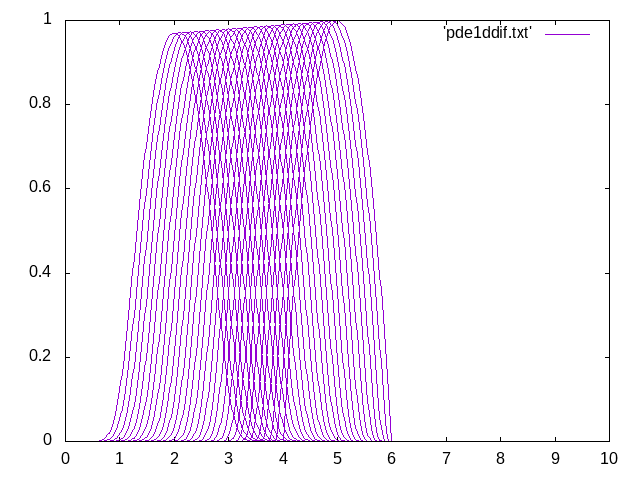
\includegraphics[width=\linewidth]{graph.png}

グラフの形は時間と共に、添付するmovie.gifのように移動していく。
頂点の値は、時間と共に減衰していく。
この減衰については、刻み幅を10分の1にして同様の計算を行うと以下のように、
ほぼ減衰が発生しないことから、
誤差により生じる減衰であることが予想される。

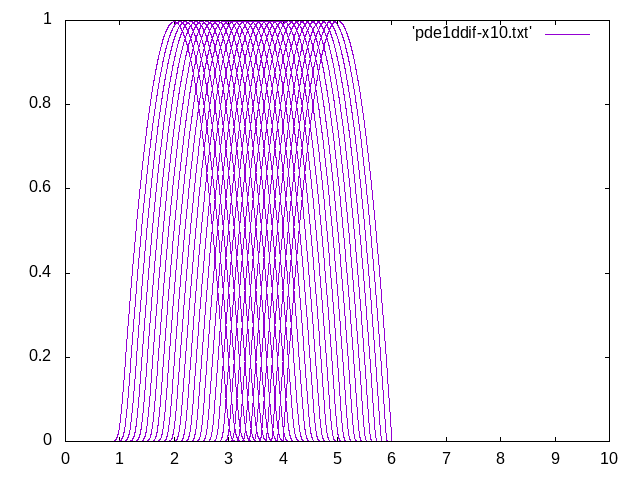
\includegraphics[width=\linewidth]{graph-x10.png}

以下のスクリプトを用いて、orbit.datから図を生成した。
\lstinputlisting[caption=plot.sh,language=bash]{plot.sh}

\end{document}
